\documentclass[./Report_main.tex]{subfiles}

% If you use beamer only pass "xcolor=table" option, i.e. 

\begin{comment}
If you want a box around your answer and that answer is an
equation then use \boxed{$$ equation $$} 

if you want to indent a block of text:
\begin{adjustwidth}{cm of right indent}{cm of left indent}
% paragraph to be indented
\end{adjustwidth}

if you just want one indent for one line 
use \indent per intended indent per line

A sections numbers automatically, so if the number of 
the problem is out of order it would be easier to 
just indent and bold the sections and subsections
and not use the \section{} kind of commands

\newpage makes a new page

$normal math mode$
$$Special math mode$$

to include an image use
\includegraphics{image_name}
image_name is the file name (.png) without the extension. The file
name cannot have any spaces or any periods other than the one before
the file extension.

To include a codeblock use
\begin{lstlisting}
ExampleCode(blah, blah)
{
	it does tabbing and everything;
	for (coloring of major languages like java){
		add the folloing to the \lstset tuple:
			language=<name_of_language>;
	}
}
\end{lstlisting}

\end{comment}


\begin{document}

%\tableofcontents

%\thispagestyle{empty}
%\newpage
% If you want to change how the subsubsection's are numbered
%\renewcommand{\thesubsection}{\thesection.\alph{subsection}.} 

%\setcounter{page}{0}
\chapter{Project plan}
\section{planning process}
In the begining of the project we defined the behaviors together, came up with an implementation plan and defined the grammars. In Github we kept track of a project management software, which we kept up to date until the hello world assignment was due. After that point instead of meticulously keeping track of the tracking system, we instead would set weekly goals at our meetings and then we would split off into teams of two and acheive the goals that we had set for eachoher for the week. Every team member brought up to speed with what had been completed and worked on durring the week at our weekly meetings. All goals for the project were put on Github either in the wiki or in the project management software and they were resolved cleared independently or in teams of two. We created several milestones which captured our goals for completing the parser, scanner, analyzer, and codegen up until the hello world assignment, and after we moved to the wiki or word of mouth at our weekly meetings. We worked weekly with Professor Edwards to receive guidance on how best to implement our language.
\section{Style guide}
We adhered to the following style guide as much as possible:\\
\begin{adjustwidth}{1cm}{}
$ \cdot $\ No lines greater than 80 characters\\
$ \cdot $\ Ensure that pattern matches are on the same indent with respect to each other\\
$\cdot $\ Use tabbed indentation as opposed to spaces. Ensure that the tab width is 4 spaces.
\end{adjustwidth}
\section{Time line}
% Please add the following required packages to your document preamble:
% \usepackage[table,xcdraw]{xcolor}
% If you use beamer only pass "xcolor=table" option, i.e. \documentclass[xcolor=table]{beamer}
\begin{lstlisting} 
Date Complete	| Event Completed
---------------------------------------------------------------------------------
02/08/2017		| Language Proposal Complete
02/22/2017		| Language Reference Manual Completed
03/20/2017		| Compiler Frontend v1.0 (Scanner, Parser, and Codegen) Complete
03/22/2017		| Hello World Runs
04/26/2017		| Testing suite v1.0 completed
05/09/2017		| Final version of the semantic checker completed
05/09/2017		| Final features added to the codegen
05/09/2017		| Final Version of the compiler complete
05/10/2017		| Final version of test suite completed
05/10/2017		| Final Report completed and turned in
\end{lstlisting}
\section{Team Responsibilities}
\begin{tabu} to 1\textwidth { | X[c] | X[c] | }
 \hline
 Team Member & Responsibility \\ 
 \hline
 Brandon Bakhshai & Libuv architecture, codegen, lists, pipes, listen (server functionality), http routing, demo program (Alexa skill), grammars, test framework (pipeline.ml file).
\\
 \hline
Ben Lai  & Grammars, Parser, ast , Codegen, writing test cases and expected output, implementation of primitives,control structure, functions, string(stdlib), List(stdlib), maintaining the translator structure(make sure all components work together), responsible for test-plan, tutorial, and appendix in the final report.
\\
 \hline
Jeffrey Serio  & Grammars, codegen, Semantic Checker, LRM, semantic check-cases and code clean-up, implementation of fileIO, and struct
\\
\hline
Somya Vasudevan & Test framework and script, codegen, http routing, pipes, demo program (Alexa skill), listen (server functionality).\\
\hline
\end{tabu}
\section{Development environment}
From the beginning of the project we agreed to the following development environment with the following software versions:
\begin{itemize}
\item \textbf{Ubuntu 16.04} - Very simple to use linux distribution that had the LLVM software and OCaml
software easily accessible. Ubuntu was used within Virtualbox to ensure consistency across hardware
as well.\\
\item \textbf{C} - The latest version of the C programming language\\
\item \textbf{gcc} - The latest version of the gcc compiler for compiling the translated pipeline code.\\
\item \textbf{OCaml} - version 4.02-3 as our primary translation environment\\
\item \textbf{Slack} - We agreed that the Slack chat messaging platform was the most convenient and efficient way to share code snippets and communicate.
\item \textbf{Github} - In order to version control our software and maintain a working version at any time, we used Github as our go to source code repository. It made integration with the team simpler and everyone was able to view the repository conveniently in their browser.//
\item \textbf{Latex} - In order to compile the documentation we made sure to all use Latex to ensure high quality material being produced for the project.//
\item \textbf{Vim} - We used vim as our primary text editor throughout the project.//
\end{itemize}
\section{Project log}
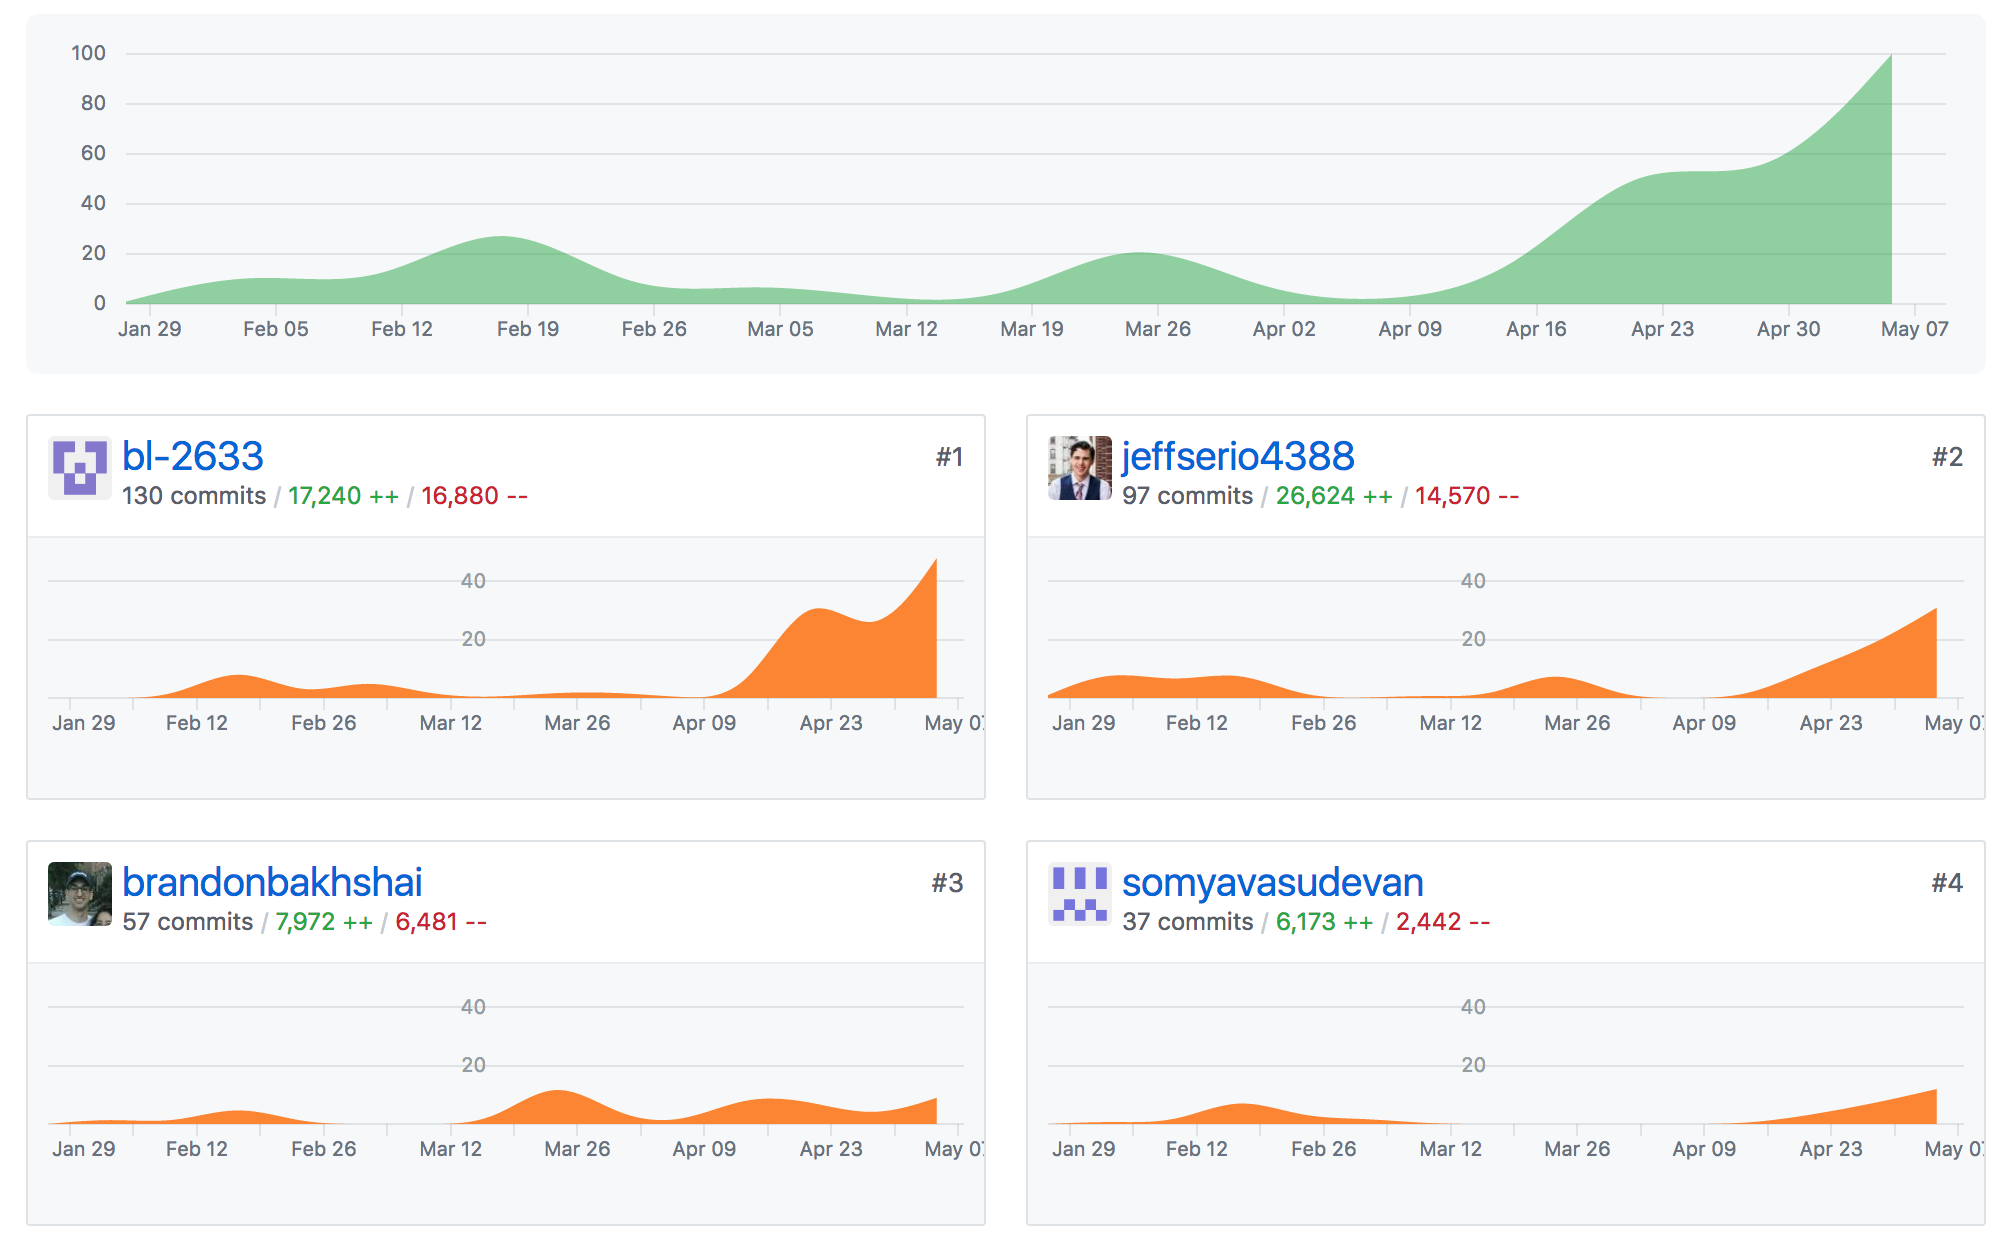
\includegraphics[scale = 0.5]{github_stats.png}
\lstinputlisting[]{./git_log.txt}
%\section{}
%\subsection{Identifiers}
%\subsubsection{}
%\subsection{subsection}
%\subsubsection{subsubsection}
\end{document}

